\subsection{Using the Georeferencer Plugin}

The georeferencer plugin allows to generate world files for rasters. Therefore
you select points on the raster, add their coordinates, and the plugin will 
compute the world file parameters. The more coordinates you provide the better 
the result will be.

As an example we will generate a world file for a topo sheet of South Dakota 
from SDGS. It can later be visualized together with in the data of the GRASS 
spearfish60 location. You can download the topo sheet here: \\
\url{http://grass.itc.it/sampledata/spearfish\_toposheet.tar.gz}

As a first step we download the file and untar it.

\begin{verbatim}
wget http://grass.itc.it/sampledata/spearfish_toposheet.tar.gz
tar xvzf spearfish_toposheet.tar.gz
cd spearfish_toposheet
\end{verbatim}

The next step is to start QGIS, load the georeferencer plugin and select 
the file spearfish\_topo24.tif.

\begin{figure}[ht]
\begin{center}
  \caption{Select an image to georeference}\label{fig:select_image}\smallskip
  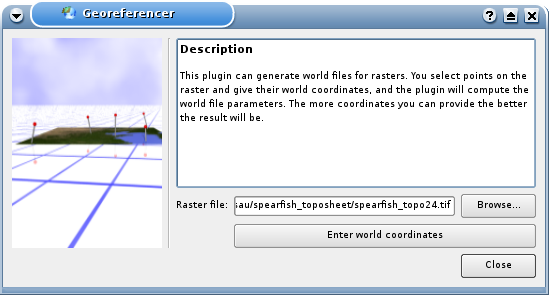
\includegraphics[clip=true]{select_image}
\end{center}
\end{figure}

Now click on the button \textsl{Arrange plugin window} to open the image 
in the georeferencer and to arrange it with the reference map in the qgis map canvas on your dekstop.

\begin{figure}[ht]
\begin{center}
  \caption{Arrange plugin window with the qgis map canvas}\label{fig:georeferencer}\smallskip
  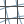
\includegraphics[clip=true,width=\textwidth]{georeferencer}
\end{center}
\end{figure}

With the button \textsl{Add Point} you can start to add points on the 
raster image and enter their coordinates, and the plugin will compute the 
world file parameters (see figure \ref{fig:choose_points}). The more coordinates you provide the better the 
result will be. For the procedure you have two option. 

\begin{enumerate}
\item You click on a point in the raster map and enter the X and Y 
coordinates manually
\item You click on a point in the raster map and choose the button
\textsl{from map canvas} to add the X and Y coordinates with the help 
of a georeference map already loaded in QGIS.
\end{enumerate}

\begin{figure}[ht]
\begin{center}
  \caption{Add points to the raster image}\label{fig:choose_points}\smallskip
  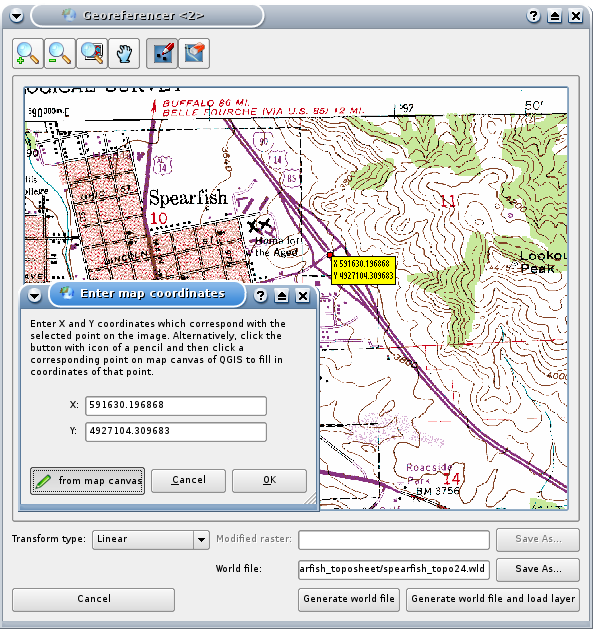
\includegraphics[clip=true,width=0.8\textwidth]{choose_points}
\end{center}
\end{figure}

For this example we use the second option and enter the coordinates for the
selected points with the help of the \textsl{roads} map provided with the 
\textsl{spearfish60} location from: \\
\url{http://grass.itc.it/sampledata/spearfish\_grass60data-0.3.tar.gz}

If you don't know how to integrate the spearfish60 location with the GRASS plugin, 
information are provided in Section \ref{sec:grass}. 

As you can see in Figure \ref{fig:choose_points}, the georeferencer provides buttons 
to zoom, pan, add and delete points in the image.   

After you added enough points to the image you need to select the transformation 
type for the georeferencing process and save the resulting world file together with 
the Tiff. In our example we choose linear transformation although a helmert 
transformation might be sufficient as well. 

\begin{Tip}\caption{\textsc{Choosing the transformation type}}
\qgistip{The linear (affine) transformation is a 1st order transformation and used 
for scaling, translation and rotation of geometrically correct images. With the 
helmert transformation you simply add coordinate information to the image like 
geocooding. If your image is contorted you will need to use software that provides 
2nd or 3rd order polynomial transformation, e.g. GRASS GIS.
}
\end{Tip} 

The points we added to the map will be stored in a \textsl{spearfish\_topo24.tif.points} file together 
with the raster image. This allows us to reopen the georeferencer plugin and to add new or delete 
existing points to optimize the result. The \textsl{spearfish\_topo24.tif.points} file of this 
example shows the points:

\begin{verbatim}
mapX    		mapY    		pixelX  pixelY
591630.196867999969982  4927104.309682800434530 591647  4.9271e+06
608453.589164100005291  4924878.995150799863040 608458  4.92487e+06
602554.903929700027220  4915579.220743400044739 602549  4.91556e+06
591511.138448899961077  4915952.302661700174212 591563  4.91593e+06
602649.526155399973504  4919088.353569299913943 602618  4.91907e+06
\end{verbatim} 

We used 5 coordinate points to georeference the raster image. To get correct results 
it is important to disperse the points regulary in the image. Finally we check the result and load 
the new georeferenced map \textsl{spearfish\_topo24.tif} and overlay it with the map \textsl{roads} 
of the spearfish60 location.

\begin{figure}[ht]
\begin{center}
  \caption{Georeferenced map with overlayed roads from spearfish60 location}\label{fig:result_map}\smallskip
  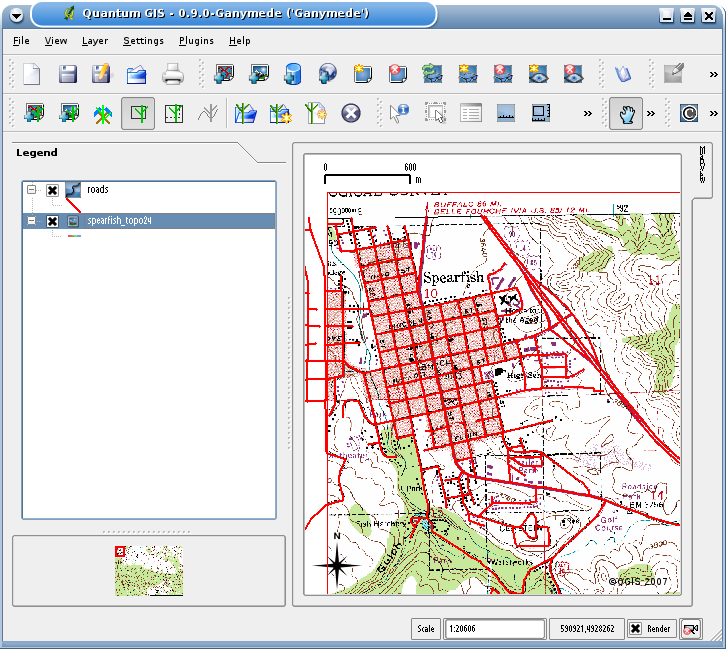
\includegraphics[clip=true,width=0.8\textwidth]{result_map}
\end{center}
\end{figure}







